\chapter{Metodología}

En este apartado describiremos la metodología utilizada para la creación del proyecto. Una metodología es un conjunto de procesos, métodos y prácticas llevadas a cabo para asegurar, en la mayor medida posible, calidad en el producto final y en el tiempo acordado.

En nuestro caso, al ser un proyecto realizado por una sola persona y con un tiempo diario limitado, hemos optado por adaptar una serie de ideas y valores principales de varias metodologías para optimizar los pocos recursos que disponemos.

\section{Desarrollo en cascada}

El desarrollo en cascada, también denominado como modelo en cascada, es una metodología con varias etapas donde, para pasar a la siguiente, es completamente necesario que la anterior haya acabado y haya sido completada en su totalidad.

Las ventajas que ofrece en desarrollo en cascada es que es muy sencillo de implementar en comparación con otras metodologías, requiere menos tiempo y capital para hacerlo funcionar de manera óptima y es usado con bastante frecuencia, por lo que sus problemas y beneficios son conocidos de antemano y, gracias a ello, podemos planear las posibles dificultades que nos puede dar. La mayor de estas desventajas es que detectar un error en una de las fases finales puede significar tener que replantear los pasos tomados en las anteriores, perdiendo parte del progreso realizado. Incluso un pequeño cambio puede llegar a afectar otras partes del análisis o diseño y nos forzará a rehacer y perder parte del trabajo hecho. 

\subsection{Etapas del desarrollo en cascada}

\paragraph{Análisis de requisitos}: 

En esta fase se definen y determinan los requisitos que el \textit{software} debe de cumplir entre el desarrollador y el cliente. Generalmente se generan documentos que formalizan dichas decisiones para no tener que cambiarlos en el futuro, dado que un cambio en los requisitos puede significar cambiar gran parte del proyecto, tal y como acabamos de comentar, por lo que llegar a un consenso es necesario.

\paragraph{Diseño}: 

Una vez del análisis haya finalizado, es hora del diseño. La idea principal es descomponer lo detallado durante el análisis de requisitos con el cliente y crear diferentes diagramas y diseños que ayuden a los programadores a entender lo que debe de ser realizado y cómo debe de funcionar, incluyendo pseudocódigo o algoritmos de alto nivel en caso de que sea necesario.

\paragraph{Implementación}:

En esta fase es donde se escribe el código fuente en base a lo especificado anteriormente, intentando dar gran importancia a la reutilización del código siempre y cuando sea posible. También es importante tener en cuenta la creación de tests y la realización de las primeras pruebas preliminares por parte de los programadores.

\paragraph{Verificación}:

Este es el momento final en el que el cliente es capaz de probar lo desarrollado. El programa debe de estar bien testado por parte de los programadores para evitar la mayoría de los problemas que pueden ocasionarse en esta fase.

\paragraph{Mantenimiento}:

Una vez el software ha finalizado y se ha entregado al usuario final, empieza la fase de mantenimiento. En ella el usuario pedirá que se resuelvan problemas, se añadan nuevas funcionalidades y se cambien otras características ya añadidas en base a los nuevos requisitos que vayan apareciendo o funcionalidades que sean necesarias y no se tuvieran en cuenta en las anteriores fases del desarrollo. Esta es una de las fases más críticas, dado que se estima que alrededor de un 80\% de los recursos de un proyecto se emplean en el mantenimiento \footnote{\url{http://eu.wiley.com/WileyCDA/WileyTitle/productCd-0471170011.html}}.

\begin{figure}[H]
		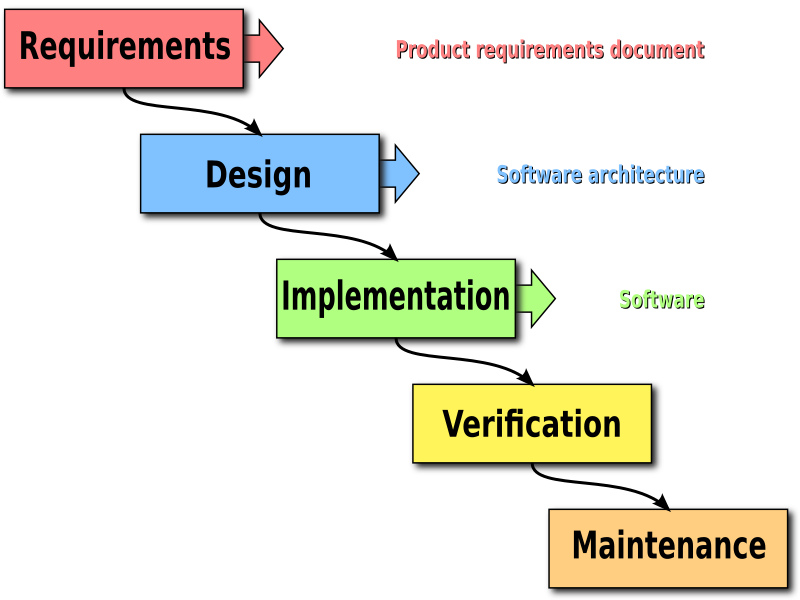
\includegraphics[width=\textwidth,height=\textheight,keepaspectratio]{./img/Waterfall_model.png}
	\caption{Estructura general de una etapa del desarrollo en cascada}
	\label{fig:cascadadesarrollo}
\end{figure}

\section{Scrum}

Scrum es una metodología ágil definida inicialmente por Hirotaka Takeuchi y Ikujiro Nonaka en 1986 \footnote{\url{https://cb.hbsp.harvard.edu/cbmp/product/86116-PDF-ENG}}. Su relativa sencillez, así como su flexibilidad y orientación al trabajo en equipo, hace que Scrum sea una de las metologías más usadas en el desarrollo de software, sobre todo en entornos laborales donde el equipo de desarrollo consta de un equipo de menos de 10 personas, aunque su implementación también es posible en estos casos, generalmente dividiendo el equipo en pequeños grupos y manejándolos de forma independiente.

\subsection{Prácticas recomendadas y bases de Scrum}

Uno de los aspectos esenciales de scrum es el ``sprint'', que se trata de un bloque temporal (comúnmente de entre 2 y 4 semanas) donde el equipo de desarrollo trabajará para llegar a un objetivo determinado, que generalmente se trata de acabar todas las tareas definidas para ese sprint. 
Al principio de cada sprint  el ``product owner'' y ``scrum master'', junto con el equipo de programadores, definirán lo necesario a realizar en dicho sprint en base a las tareas que se encuentran en el backlog\footnote{Lista de tareas que se quieren realizar en el producto y que suele ir creciendo a medida que los usuarios encuentran fallos o necesitan nuevas funcionalidades. Normalmente el \textit{product owner} es el encargado de organizar y decidir aquellas que tienen más prioridad}. Todos los integrantes del grupo, así como el propio \textit{product owner} y \textit{scrum master}, decidirán cuánto esfuerzo o tiempo llevará realizar cada una de ellas (hay algunas formas de decidir esto, como \textit{planning poker}, pero no es muy relevante en nuestro caso), dividiéndola en tareas menores en caso de que sea demasiado grande. También se decidirá quién hará qué, aunque variaciones donde los desarrolladores las van cogiendo a medida que finalizan en las que han estado trabajando\footnote{Algunas compañias llevan Scrum al límite y entrenan a sus empleados para que puedan realizar cualquier tipo de tarea sin limitaciones, por lo que esto es algo que funcionaría muy bien en situaciones similares}. De esta manera no todas las tareas tienen un responsable al inicio del \textit{sprint}.

Durante cada día del desarrollo hay una pequeña reunión llamada ``sprint stand-up'' donde cada uno de los programadores comenta brevemente lo que ha hecho el día anterior, qué tiene planteado realizar ese día y si se ha encontrado con algún problema que le impida continuar.

Al acabar cada sprint, el equipo se reúne de nuevo para analizar lo que ha ido bien, qué problemas hubo y las mejoras que deben de aplicarse y tener en cuenta de cara al futuro, así como un resumen de estadísticas del equipo en general como la \textit{burn down chart}. De esta manera, cada nuevo sprint será más preciso (dado que sabremos la cantidad de trabajo que el equipo de desarrollo es capaz de hacer en el periodo definido de tiempo) e incluirán el ``feedback'' de los propios programadores para que su trabajo diario sea más llevadero.

Estas son las características eseciales de \textit{Scrum}, pero al tratarse de una metodología ágil, nada es inamovible y existen bastantes variaciones (como la inclusión de otras metodologías como \textit{Kanban}) que se adaptan a todo tipo de equipos. Dependiendo de la empresa, equipo y necesidades del mismo, se pueden cambiar o introducir nuevas ideas que mejoren el proceso para ese grupo de trabajadores y empresa en concreto.

\begin{figure}[H]
		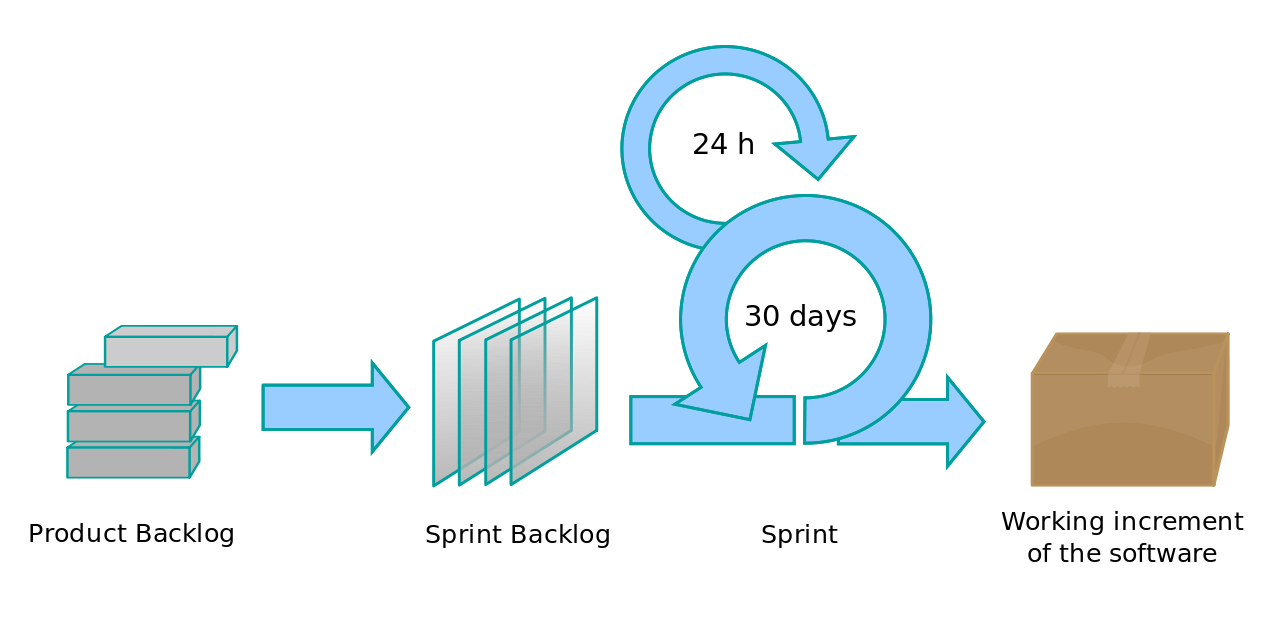
\includegraphics[width=\textwidth,height=\textheight,keepaspectratio]{./img/scrumprocess.png}
	\caption{Proceso concreto de \textit{Scrum}. En este caso el sprint dura 4 semanas}
	\label{fig:scrumproceso}
\end{figure}

\subsection{Valores de \textit{Scrum}}

\textit{Scrum} se basa en flexibilidad y trabajo en equipo. Este es el motivo por el que es muy importante tener un equipo que tenga claro y cumpla con una filosofía y valores básicos. Estos valores son los siguientes:

\subsubsection{Concentración}

Al tener que finalizar las tareas asignadas al final del \textit{sprint}, la concentración del equipo en general y de cada uno de los miembros en particular, es esencial. Para logar este objetivo, el \textit{product owner} es el encargado de responder las preguntas del resto de la compañía en nombre de los desarrolladores y solamente molestarlos en caso de que sea realmente necesario. Hay varios elementos asociados a \textit{Scrum} que ayudan a resolver este problema.

\subsubsection{Coraje}

Dado que \textit{Scrum} es una metodología de equipo, la ayuda entre cada uno de los miembros es primordial. De igual modo, cada persona debe de ser capaz de enfrentarse a nuevos retos y asumir nuevas responsabilidades para que, en conjunto, el producto final sea el deseado. 

\subsubsection{Compromiso}

Cada integrante tiene que saber lo que puede hacer y comprometerse a ello. Una vez la reunión inicial se haya completado, es importante que cada desarrollador sepa en lo que tiene que trabajar y pregunte al responsable de la tarea en caso de que no tenga algo claro o crea que no puede llegar a terminar lo acordado durante la reunión. Cada programador debe de comprometerse con lo establecido para lograr el éxito del equipo.

\subsubsection{Sinceridad}

Ser capaz de asumir los errores personales y del propio equipo es la clave para mejorar y evolucionar. Si un miembro del equipo de desarrollo se queda estancado en un problema y no avisa al resto de sus compañeros, el \textit{sprint} en su totalidad puede llegar a fracasar por su culpa. Asumir responsabilidades, errores y pedir ayuda cuando sea necesario debe de ser una práctica habitual para que esta metodología funcione sin problemas.

\subsubsection{Respeto}

Similar al anterior punto. Al trabajar en equipo es imprescindible que tanto los logros como los fracasos se tomen como una nueva forma de aprender y mejorar, por lo que el respeto mutuo y asumir los fallos cometidos durante la iteración es la mejor forma de evolucionar, tanto individualmente como en equipo.

\section{Metodología elegida}
\label{sec:metodologiaelegida}

Mayoritariamente hemos usado una metodología en cascada con algunos elementos de \textit{Scrum} y otras metodologías y prácticas relacionadas.

Para las características grandes del proyecto como la creación de los mapas, enemigos, sistema creación de frases, etc. nos hemos basado en cascada para analizar lo que tenemos que realizar, crear el diseño, implementarlo (empezando siempre por los tests, tal y como comentaremos a continuación) y verificarlo. Sin embargo, y dado que los juegos tienden a querer mejorarse continuamente con nuevos elementos de diferente importancia y tamaño (tanto de nuestra parte como de la gente que lo ha probado), tiene sentido mantener un \textit{backlog} con todas las nuevas ideas que vayamos recibiendo y \textit{feedback} recogido, algo de lo que \textit{Scrum} es maestro. 
También hemos seguido la idea de la creación de tareas cortas y \textit{sprints}, donde en cada una de las iteraciones intentaremos tener un elemento del juego finalizado, siempre y cuando nuestras estimaciones iniciales no se vean comprometidas. De esta manera seremos capaces de seguir más fácilmente el progreso que hemos realizado y tenemos constancia de los nuevos elementos que queremos implementar en un futuro, así como los bugs que arreglar en próximos \textit{sprints}.
Al acabar con el núcleo del juego, la mayor parte de las tareas a realizar a continuación son pequeños cambios y nuevos elementos que no trastocan el diseño realizado del proyecto, por lo que seguir una metodología ágil como \textit{Scrum} es el mejor paso a seguir para terminar las tareas más relevantes lo antes posible. Además, el juego en sí lo hemos desarrollado con la idea de hacerlo lo más ampliable y extendible posible. De esta forma, incluso aunque tengamos que cambiar algo en medio del desarrollo, las bases creadas serán sólidas y fácilmente modificables. 

Por último, también hemos seguido la práctica de \textit{test driven development} (desarrollo guiado por pruebas) cuya base está en que por cada nueva tarea a realizar, deberemos de implementar primero los tests unitarios (que, lógicamente, fallarán) y luego programar la solución en sí para que el test sea válido, refactorizando la solución en caso de que no sea la ideal. Esto nos dará desde el primer momento una idea clara de lo que queremos hacer antes de ponernos con la implementación y nos asegurará de que siempre tendremos el test hecho.